%% LyX 2.2.0 created this file.  For more info, see http://www.lyx.org/.
%% Do not edit unless you really know what you are doing.
\documentclass[english,aps, twocolumn, pre,superscriptaddress, notitlepage]{revtex4-1}
\usepackage[T1]{fontenc}
\usepackage[latin9]{inputenc}
\setcounter{secnumdepth}{3}
\usepackage{array}
\usepackage{textcomp}
\usepackage{bm}
\usepackage{amsmath}
\usepackage{amssymb}
\usepackage{graphicx}

\makeatletter

%%%%%%%%%%%%%%%%%%%%%%%%%%%%%% LyX specific LaTeX commands.
%% Because html converters don't know tabularnewline
\providecommand{\tabularnewline}{\\}

%%%%%%%%%%%%%%%%%%%%%%%%%%%%%% User specified LaTeX commands.
\usepackage[colorlinks=true,linktocpage=true,linkcolor=MidnightBlue,urlcolor=MidnightBlue,citecolor=MidnightBlue,anchorcolor=MidnightBlue]{hyperref}
\usepackage[dvipsnames]{xcolor}

\makeatother

\usepackage{babel}
\begin{document}

\title{Fast Bayesian inference of the multivariate Ornstein-Uhlenbeck process}

\author{Rajesh Singh}

\affiliation{The Institute of Mathematical Sciences-HBNI, CIT Campus, Taramani,
Chennai 600113, India}

\author{Dipanjan Ghosh}

\affiliation{Dept of Chemical Engineering, Jadavpur University, Kolkata 700032,
India}

\author{R. Adhikari}
\email{rjoy@imsc.res.in}


\affiliation{The Institute of Mathematical Sciences-HBNI, CIT Campus, Taramani,
Chennai 600113, India}

\affiliation{DAMTP, Centre for Mathematical Sciences, University of Cambridge,
Wilberforce Road, Cambridge CB3 0WA, UK}
\begin{abstract}
The multivariate Ornstein-Uhlenbeck process is used in many branches
of science and engineering to describe the regression of a system
to its stationary mean. Here we present a fast Bayesian method to
estimate the drift and diffusion matrices of the process from discretely
observed sample paths. We use exact likelihoods, expressed in terms
of four sufficient statistic matrices, to derive explicit maximum
a posteriori parameter estimates and their standard errors. We apply
the method to the Brownian harmonic oscillator, a bivariate Ornstein-Uhlenbeck
process, to jointly estimate its mass, damping, and stiffness and
to provide Bayesian estimates of the correlation functions and power
spectral densities. We present a Bayesian model comparison procedure,
embodying Ockham's razor, to guide a data-driven choice between the
Kramers and Smoluchowski limits of the oscillator. These provide novel
methods of analysing the inertial motion of colloidal particles in
optical traps. 
\end{abstract}
\maketitle

\section{Introduction}

The multivariate Ornstein-Uhlenbeck process is widely used in many
branches of science and engineering to describe the regression of
a system to its stationary mean. Its importance arises from the fact
that it is the only process that is simultaneously Markovian, Gaussian
and stationary. The process, therefore, is fully characterized by
its stationary and conditional distribution, each of which are multivariate
normal distributions. This simplicity implies that the probabilities
of discretely sampled paths can be calculated exactly and explicitly
in terms of the process parameters, the drift and diffusion matrices.
In turn, this implies an exact expression for the likelihood of paths,
given the parameters, and the possibility of exact Bayesian inference. 

Here we present the details of such an exact Bayesian estimation method
for the $M$-dimensional Ornstein-Uhlenbeck process. From the exact
likelihood of the discrete path, we identify four matrices of sufficient
statistics, in terms of which we derive MAP estimates and the error
bars of the process parameters. In addition we examine the problem
of model selection, that is, of choosing the Ornstein-Uhlenbeck model
with the least number of parameters that best explains the data. Both
these aspects are illustrated using the Brownian harmonic oscillator,
a bivariate Ornstein-Uhlenbeck process, as an example. Inter alia,
this provides a Bayesian method for estimating the mass, friction,
spring constant, correlation functions and power spectral densities
of colloidal particles in optical traps. 

The remainder of the paper is organized as follows. In section \ref{sec:mvoup},
we briefly review key properties of the Ornstein-Uhlenbeck process
and make use of them in section \ref{sec:Bayesian-inference} to obtain
MAP estimates for the parameters and the model odds. In section \ref{sec:Path-sampling}
we present an exact path sampling algorithm which is used in \ref{sec:Brownian-harmonic-oscillator}
to generate sample paths of the Brownian harmonic oscillator and to
validate the results of section \ref{sec:Bayesian-inference}. We
conclude in section \ref{sec:conclusion} with a discussion on further
applications. 

\section{Multivariate Ornstein-Uhlenbeck Process\label{sec:mvoup}}

The multivariate Ornstein-Uhlenbeck is defined by the Ito stochastic
differential equation \cite{gardiner1985handbook}

\begin{equation}
dx_{i}=-\lambda_{ij}x_{j}dt+(\sqrt{2D})_{ij}\cdot dW_{j},\label{eq:mvou}
\end{equation}
where $\lambda_{ij}$ is a stable matrix of mean regression rates,
$D_{ij}$ is a symmetric positive semi-definite matrix of diffusion
coefficients, $W_{i}(t)$ are Wiener process and $i,j=1,\ldots,M$.
We denote $(x_{1},\ldots,x_{M})^{T}$ by the vector $\boldsymbol{x}$
and $\lambda_{ij}$ by the matrix $\boldsymbol{\lambda}$, with similar
bold-face notation for other vectors and matrices, when convenient. 

The probability density of a displacement from $\boldsymbol{x}$ at
time $t$ to $\boldsymbol{x}^{\prime}$ at time $t^{\prime}$, $P_{1|1}$$(\boldsymbol{x}^{\prime}t^{\prime}|\boldsymbol{x}\thinspace t$),
obeys the Fokker-Planck equation $\partial_{t}P_{1|1}=\mathcal{L}P_{1|1}$,
where the Fokker-Planck operator is
\begin{equation}
\mathcal{L}(\boldsymbol{x})=-\frac{\partial}{\partial x_{i}}\lambda_{ij}x_{j}+\frac{\partial^{2}}{\partial x_{i}\partial x_{j}}D_{ij}.
\end{equation}
The solution is a multivariate normal distribution
\begin{equation}
\mathbf{\boldsymbol{x}}^{\prime}t^{\prime}|\boldsymbol{x}\thinspace t\sim\mathcal{N}\left(\boldsymbol{\mu}\,,\boldsymbol{\Sigma}\right),\label{eq:conditional-probability}
\end{equation}
where 
\begin{equation}
\boldsymbol{\mu}=\boldsymbol{\Lambda}\boldsymbol{x},\quad\boldsymbol{\Sigma}=\boldsymbol{c}-\boldsymbol{\Lambda}\boldsymbol{c}\,\boldsymbol{\Lambda}^{T},\quad\boldsymbol{\Lambda}=e^{-\boldsymbol{\lambda}\Delta t}
\end{equation}
and $\Delta t=t'-t$. This solution is exact and holds for arbitrary
values of $|\Delta t|$. The stationary distribution $P_{1}(\boldsymbol{x})$
obeys the steady state Fokker-Plank equation $\mathcal{L}P_{1}=0$
and the solution is, again, a normal distribution,
\begin{equation}
\boldsymbol{x}\sim\mathcal{N}\left(\boldsymbol{0},\boldsymbol{c}\right).
\end{equation}
Then, $\boldsymbol{c}=\langle\boldsymbol{x}\boldsymbol{x}^{T}\rangle$
can be identified as the matrix of covariances in the stationary state
and $\mathcal{L}P_{1}=0$ implies that the matrices $\boldsymbol{\lambda}$,
$\boldsymbol{D}$ and $\boldsymbol{c}$ are not all independent but
are related by the stationarity condition
\begin{equation}
\boldsymbol{\lambda c}+(\boldsymbol{\lambda c})^{T}=2\boldsymbol{D}.\label{eq:stationarity}
\end{equation}
This is a Lyapunov matrix equation for $\boldsymbol{c},$ given $\boldsymbol{\lambda}$
and $\boldsymbol{D}$. Solutions are considerably simplified when
the Fokker-Planck operator obeys detailed balance $\mathcal{L}(\boldsymbol{x)}P_{1}(\boldsymbol{x})=P_{1}(\boldsymbol{\epsilon x})\mathcal{L}^{\dagger}(\boldsymbol{\epsilon x})$,
where $\mathcal{L^{\dagger}}$ is the adjoint Fokker-Planck operator,
$\text{\ensuremath{\boldsymbol{\epsilon}} is a diagonal matrix of the parities }\epsilon_{i}=\pm1$
of $x_{i}$ under time reversal, and the stationary distribution is
time-reversal invariant, $P(\boldsymbol{x})=P(\boldsymbol{\epsilon x})$.
This implies Onsager-Casimir symmetry $\boldsymbol{\epsilon}(\boldsymbol{\lambda c})=(\boldsymbol{\lambda c})^{T}\boldsymbol{\epsilon}$
for the regression matrix and $\boldsymbol{\epsilon c}=\boldsymbol{c\epsilon}$
for the covariance matrix.

The Gauss-Markov property of the Ornstein-Uhlenbeck process ensures
that the correlation function
\begin{equation}
\boldsymbol{C}(t-t^{\prime})\equiv\langle\boldsymbol{x}(t)\boldsymbol{x}^{T}(t^{\prime})\rangle=e^{-\boldsymbol{\lambda}|\Delta t|}\boldsymbol{c},\mathbf{}\label{eq:autocorr}
\end{equation}
decays exponentially and that its Fourier transform, the power spectral
density
\begin{equation}
\boldsymbol{C}(\Omega)=(\text{\textminus}i\Omega\boldsymbol{1}+\boldsymbol{\lambda})^{-1}\left(2\boldsymbol{D}\right)(i\Omega\boldsymbol{1}+\boldsymbol{\lambda^{T}})^{-1},\label{eq:spectral-density}
\end{equation}
is a multivariate Lorentzian in the angular frequency $\Omega$ \cite{van1992stochastic}. 

In what follows, we shall take $\boldsymbol{\Lambda}$, the matrix
exponential of the mean regressions rates and $\boldsymbol{c}$, the
covariance matrix, to be the independent parameters. Estimates of
the parameters in the diffusion matrix can then be obtained from the
estimates of $\boldsymbol{\Lambda}$ and $\boldsymbol{c}$ through
the stationarity condition. For notational brevity the set of all
unknown parameters is collected in $\boldsymbol{\theta}=(\boldsymbol{\Lambda},\boldsymbol{c})$. 

\section{Bayesian inference\label{sec:Bayesian-inference}}

\emph{Parameter Estimation: }Consider now the discrete time series
$\boldsymbol{X}=\left(\boldsymbol{x}_{1},\boldsymbol{x}_{2},...,\boldsymbol{x}_{N}\right)$,
consisting of $N$ observations of the sample path $\boldsymbol{x}(t)$
at the discrete times $t=n\Delta t$ with $n=1,\ldots,N.$ Each observation
$\boldsymbol{x}_{n}$ is an $M$-dimensional vector corresponding
to the number of components of the multivariate Ornstein-Uhlenbeck
process. From the Markov property of the process, the probability
of the path, given the parameters in $\boldsymbol{\theta}$, is
\begin{equation}
P\left(\boldsymbol{X}\vert\boldsymbol{\theta}\right)=\prod_{n=1}^{N-1}P_{1\vert1}\left(\boldsymbol{x}_{n+1}\vert\boldsymbol{x}_{n},\boldsymbol{\theta}\right)P_{1}\left(\boldsymbol{x}_{1}\vert\boldsymbol{\theta}\right).
\end{equation}
The probability $P\left(\boldsymbol{\theta}\vert\boldsymbol{X}\right)$
of the parameters, given the sample path, is given by Bayes theorem
to be
\begin{equation}
P\left(\boldsymbol{\theta}\vert\boldsymbol{X}\right)=\dfrac{P\left(\bm{X}\vert\boldsymbol{\theta}\right)P\left(\boldsymbol{\theta}\right)}{P\left(\boldsymbol{X}\right)}.\label{eq:bayes-theorem}
\end{equation}
The denominator $P\left(\bm{X}\right)$ is a normalization independent
of the parameters and can, so, be ignored in parameter estimation.
Using informative uniform priors for $P\left(\boldsymbol{\theta}\right)$,
the logarithm of the posterior probability, after using the explicit
forms of $P_{1\vert1}$ and $P_{1}$, is
\begin{align*}
\ln P\left(\boldsymbol{\theta}\vert\bm{X}\right) & =-\frac{1}{2}\sum_{n=1}^{N-1}\boldsymbol{\Delta}_{n}^{T}\boldsymbol{\Sigma}^{-1}\boldsymbol{\Delta}_{n}-\dfrac{1}{2}\boldsymbol{x}_{1}^{T}\boldsymbol{c}^{-1}\,\boldsymbol{x}_{1}\\
 & +\dfrac{N-1}{2}\ln\dfrac{1}{\left(2\pi\right)^{M}\vert\bm{\Sigma}\vert}+\dfrac{1}{2}\ln\dfrac{1}{\left(2\pi\right)^{M}|\bm{c}|}
\end{align*}
where 
\begin{align}
\boldsymbol{\Delta}_{n} & \equiv\boldsymbol{x}_{n+1}-\boldsymbol{\Lambda}\,\boldsymbol{x}_{n}.\label{eq:posteriorBayesI}
\end{align}
With some elementary manipulations, detailed in the Appendix, the
posterior probability can be written in terms of the following four
matrix sufficient statistics \begin{subequations}\label{eq:sufficientStatistics}
\begin{flalign}
\boldsymbol{T}_{1} & =\sum_{n=1}^{N-1}\boldsymbol{x}_{n+1}\boldsymbol{x}_{n+1}^{T},\quad\boldsymbol{T}_{2}=\sum_{n=1}^{N-1}\boldsymbol{x}_{n+1}\boldsymbol{x}_{n}^{T},\\
\boldsymbol{T}_{3} & =\sum_{n=1}^{N-1}\boldsymbol{x}_{n}\boldsymbol{x}_{n}^{T},\quad\quad\quad\boldsymbol{T}_{4}=\boldsymbol{x}_{1}\boldsymbol{x}_{1}^{T}.
\end{flalign}
\end{subequations}and the maximum a posteriori (MAP) estimates for
mean regression rates and the covariances come out to be\begin{subequations}\label{eq:mapBayesI}
\begin{align}
\bm{\bm{\Lambda}^{\ast}} & =\bm{T}_{2}\boldsymbol{T}_{3}^{-1},\label{eq:map_lambda}\\
\bm{\Sigma^{\ast}} & =\dfrac{1}{N}\left(\bm{T}_{1}-\boldsymbol{T}_{2}\boldsymbol{T}_{3}^{-1}\boldsymbol{T}_{2}^{T}\right).\label{eq:map_sigma}
\end{align}
\end{subequations}The standard errors are obtained from the Hessian
matrix $\bm{A}$ of the posterior probability evaluated at the maximum
\cite{jeffreys1998theory,jaynes2003probability,sivia2006data}. Its
explicit form is provided in the Appendix. The four $M\times M$ sufficient
statistic matrices $\boldsymbol{T}_{i}$ rather than the considerably
larger $M\times N$ times series $\boldsymbol{X}$ contains all the
information relevant for inference. Their use reduces both the storage
and computational cost of the inference algorithm. 

The estimate for the mean regression rate is easily recognized to
be the multivariate generalization of our earlier result for the univariate
Ornstein-Uhlenbeck process \cite{bera2017fast}. An explicit estimate
for $\boldsymbol{c}$ can be obtained from that of $\boldsymbol{\Sigma}$
when the Fokker-Planck operator obeys detailed balance. Then Onsager-Casimir
symmetry $\boldsymbol{\epsilon}(\boldsymbol{\lambda c})=(\boldsymbol{\lambda c})^{T}\boldsymbol{\epsilon}$
implies $\boldsymbol{\Lambda}\boldsymbol{c}=\boldsymbol{c}\boldsymbol{\epsilon}\boldsymbol{\Lambda}^{T}\boldsymbol{\epsilon}$
and, from the definition of $\boldsymbol{\Sigma}$, it follows that
the MAP estimate for $\boldsymbol{c}$ is
\begin{equation}
\boldsymbol{c}^{\ast}=\boldsymbol{\Sigma}^{\ast}\left[\boldsymbol{1}-(\boldsymbol{\Lambda}^{\ast}\boldsymbol{\epsilon})^{T}(\boldsymbol{\Lambda}^{\ast}\boldsymbol{\epsilon})^{T}\right]^{-1}.\label{eq:covariance-OC}
\end{equation}
The MAP estimate for the matrix of diffusion coefficients then follows
from the stationarity condition. This is the multivariate generalization
of our earlier result for the diffusion coefficient for the univariate
Ornstein-Uhlenbeck process. We refer to this method as ``Bayes I'',
following the terminology of \cite{bera2017fast}.

In the absence of detailed balance such explicit expressions can no
longer be found and linear systems have to be solved to obtain the
MAP estimate of $\boldsymbol{c}$ from that of $\boldsymbol{\Sigma}$
and, then, to relate it to the matrix of diffusion coefficients. We
shall pursue this elsewhere. 

An alternative Bayesian procedure for directly estimating $\boldsymbol{c}$
is arrived at by interpreting the time series $\boldsymbol{X}$ as
independent repeated samples from the stationary distribution $\mathcal{N}\left(\boldsymbol{0},\boldsymbol{c}\right)$.
Using non-informative priors, the expression of the logarithm of the
posterior probability in this approach is given as
\begin{align}
\ln P\left(\boldsymbol{c}\,|\boldsymbol{X}\right) & =\dfrac{N}{2}\ln\dfrac{1}{\left(2\pi\right)^{M}|\bm{c}|}-\dfrac{1}{2}\sum_{n=1}^{N}\boldsymbol{x}_{n}^{T}\boldsymbol{c}^{-1}\,\boldsymbol{x}_{n},\label{eq:posteriorBayesII}
\end{align}
from which the MAP estimate
\begin{align}
\boldsymbol{c}^{\ast}=\frac{1}{N}\sum_{n=1}^{N}\boldsymbol{x}_{n}\boldsymbol{x}_{n}^{T}=\frac{1}{N}\boldsymbol{T}_{3},\label{eq:mapBayesII}
\end{align}
follows straightforwardly. The Bayesian inference method described
above, using the stationary distribution of the Ornstein-Uhlenbeck
process, is referred to as \textquotedblleft Bayes II\textquotedblright .
Consistency between the above two methods of estimating the covariance
matrix provides a stringent test of the appropriateness of the Ornstein-Uhlenbeck
process as the data generating model. The preceding equations (\ref{eq:mapBayesI}),
(\ref{eq:covariance-OC}) and (\ref{eq:mapBayesII}) are the central
results of this paper.

\emph{Model comparison: }Thus far we assumed that the data generating
model was given and that only the parameters of the model needed to
be estimated. In certain circumstances, though, the model itself may
be uncertain and it becomes necessary to estimate the probability
of different models $\mathcal{M}_{\alpha}$ \cite{jeffreys1998theory,kashyap1977bayesian,mackay1992bayesian,zellner1984,gregory2005bayesian}.
The probability of a model, given the data, is
\begin{equation}
P(\mathcal{M}_{\alpha}|\boldsymbol{X})\propto P(\boldsymbol{X}|\mathcal{M}_{\alpha})P(\mathcal{M}_{\alpha}),
\end{equation}
where the first term on the right is the ``evidence'' of the model
and the second term is the prior probability of the model. We shall
assume all models to be, a priori, equally likely. The evidence is
the normalizing constant in Eq.(\ref{eq:bayes-theorem}), given as
an integral over the space of parameters $\boldsymbol{\theta}$ contained
in the drift and diffusion matrices:
\begin{equation}
P(\boldsymbol{X}|\mathcal{M}_{\alpha})=\int P(\boldsymbol{X}|\boldsymbol{\theta},\mathcal{M}_{\alpha})P(\boldsymbol{\theta}|\mathcal{M}_{\alpha})d\boldsymbol{\theta}.
\end{equation}
For unimodal posterior distributions, the height at the MAP value
$\boldsymbol{\theta}^{\ast}$ times the width $\Delta\boldsymbol{\theta}$
of the distribution is, often, a very good approximation for the evidence,
\begin{equation}
P(\boldsymbol{X}|\mathcal{M}_{\alpha})\simeq P(\boldsymbol{X}|\boldsymbol{\theta}^{\ast},\mathcal{M}_{\alpha})P(\boldsymbol{\theta}^{\ast}|\mathcal{M}_{\alpha})\Delta\boldsymbol{\theta}.\label{eq:evidence}
\end{equation}
The first term is the best fit likelihood while the second term, the
product of the prior for the MAP estimate and the standard error of
this estimate is called the Ockham factor. Thus models which achieve
a compromise between the degree of fit to the data and the number
of parameters required for the fit are ones which are favoured by
the Bayesian model selection procedure. This avoids the over-fitting
that would occur if the degree of fit was made the sole criterion
for model selection and encodes the commonsense ``principle of parsimony'',
 attributed to William of Ockham, that between two models that fit
the data equally well, the simpler one is to be preferred. Both the
evidence and the Ockham factor can be obtained straightforwardly for
the Ornstein-Uhlenbeck models and we shall make use of this below
for model selection within a family of Ornstein-Uhlenbeck models. 

\section{Path sampling\label{sec:Path-sampling}}

The solution of the Fokker-Planck equation, Eq.(\ref{eq:conditional-probability}),
provides a method for sampling paths of the multivariate Ornstein-Uhlenbeck
process \emph{exactly}. Given an initial state $\boldsymbol{x}$ at
time $t$ and final state $\boldsymbol{x}^{\prime}$ at time $t^{\prime}$
, the quantity $\boldsymbol{x}^{\prime}-\boldsymbol{\Lambda}\boldsymbol{x}$
is normally distributed with mean zero and variance $\boldsymbol{\Sigma}$,
a property that was first recognized by Uhlenbeck and Ornstein. Therefore,
a sequence of states at times $t=n\Delta t$, where $n$ is a positive
integer, forming a discrete sampling of a path can be obtained from
the following iteration \cite{uhlenbeck1930theory}
\begin{equation}
\boldsymbol{x}_{n+1}=\boldsymbol{\Lambda}\boldsymbol{x}_{n}+\sqrt{\boldsymbol{\Sigma}}\,\boldsymbol{\xi}_{n},\label{eq:path-sampling}
\end{equation}
where $\sqrt{\boldsymbol{\Sigma}}$ is a matrix square-root of $\boldsymbol{\Sigma}$
and $\boldsymbol{\xi}_{n}\sim\mathcal{N}(\boldsymbol{0},\boldsymbol{1})$
is an $M$-dimensional uncorrelated normal variate with zero mean
and unit variance. The exponential of the regression matrix and the
square-root of the variance matrix are the two key quantities in the
iteration. They can be obtained analytically in low dimensional problems
but for high dimensional problems they will, in general, have to be
obtained numerically. The sampling interval must satisfy $\lambda_{\mathrm{max}}\Delta t\ll1$
such that the shortest time scale in the dynamics, corresponding to
the inverse of the largest eigenvalue $\lambda_{\mathrm{max}}$ of
the regression matrix, is resolved in the samples. In the following
section we use the method above to sample paths of the Brownian harmonic
oscillator, which is equivalent to a bivariate Ornstein-Uhlenbeck
process, to test the accuracy of our Bayesian estimates.

\section{Brownian harmonic oscillator\label{sec:Brownian-harmonic-oscillator}}

\emph{Inference problem: }We now apply the results above to the physically
important case of a massive Brownian particle confined in a harmonic
potential described by the Langevin equation
\begin{equation}
m\dot{v}+\gamma v+\nabla U(x)=\xi.\label{eq:langevin}
\end{equation}
Here the pair $(x,v)$ describes the state of the particle in its
phase space of position and velocity, while $m$ and $\gamma$ are
the particle mass and friction coefficient respectively. The potential
$U=\frac{1}{2}kx^{2}$ is harmonic with a stiffness $k$. $\xi\left(t\right)$is
a zero-mean Gaussian white noise with variance $\langle\xi\left(t\right)\xi\left(t'\right)\rangle=2k_{B}T\gamma\delta\left(t-t'\right)$
that satisfies the fluctuation-dissipation relation \cite{chandrasekhar1943stochastic}.
The inference problem is to jointly estimate the triplet of parameters
$(m,\gamma,k)$ from discrete observations of the position and velocity
and to estimate the correlation functions and the spectral densities
from these observations. 

\emph{Bivariate Ornstein-Uhlenbeck process: }The Langevin equation
can be recast as a bivariate Ornstein-Uhlenbeck process in phase space
\begin{equation}
d\left(\begin{array}{c}
x\\
v
\end{array}\right)=-\bm{\lambda}\left(\begin{array}{c}
x\\
v
\end{array}\right)dt+\sqrt{2\boldsymbol{D}}\left(\begin{array}{c}
dW_{x}\\
dW_{v}
\end{array}\right),\label{eq:phase_space}
\end{equation}
where the mean regression matrix is
\begin{equation}
\bm{\lambda}=\begin{pmatrix}0 & -1\\
\omega_{0}^{2} & 1/\tau
\end{pmatrix},
\end{equation}
and the diffusion matrix is
\begin{equation}
\bm{D=}\begin{pmatrix}0 & 0\\
0 & D/\tau^{2}
\end{pmatrix}.
\end{equation}
Here $\omega_{0}=\sqrt{k/m}$ is the natural frequency of the undamped
harmonic oscillator, $\tau=m/\gamma$ is the characteristic time scale
associated with the thermalization of the momentum due to viscous
dissipation, and $\omega=\sqrt{k/m-\gamma^{2}/(2m)^{2}}=\sqrt{\omega_{0}^{2}-1/(2\tau)^{2}}$
is the frequency of the damped oscillator. The diffusion coefficient
of the particle is defined, as usual, by the Einstein relation $D=k_{B}T\gamma^{-1}$
\cite{einstein1905theory,kubo1966fluctuation}. The structure of the
diffusion matrix ensures that the positional Wiener process $dW_{x}$
does not enter the dynamics. 

At thermal equilibrium, the joint distribution of position and velocity
factorize into the Gibbs distribution for the position and the Maxwell-Boltzmann
distribution for the velocity to give a diagonal covariance matrix
\begin{equation}
\bm{c}=\begin{pmatrix}k_{B}T/k & 0\\
0 & k_{B}T/m
\end{pmatrix}.\label{eq:covarianceDiagonal}
\end{equation}
It is easily verified that the stationarity condition, Eq. (\ref{eq:stationarity}),
is satisfied by the above matrices. The condition of micro-reversibility
translates, here, into Onsager-Casimir symmetry, $\boldsymbol{\lambda}^{\mathrm{ir}}\boldsymbol{c}=\boldsymbol{D}$,
where $\lambda_{ij}^{\mathrm{ir}}=\frac{1}{2}(\lambda_{ij}+\epsilon_{i}\epsilon_{j}\lambda_{ij})$
is the irreversible part of the drift coefficient with $\epsilon_{i}=\pm1$
for variables that are, respectively, even or odd under time reversal.
Then, the only non-zero entry of $\boldsymbol{\lambda}^{\mathrm{ir}}$
is $\lambda_{22}^{\mathrm{ir}}=\tau^{-1}$ and it is trivial to verify
the Onsager-Casimir symmetry.

\emph{Path sampling: }To sample paths of the Brownian harmonic oscillator
exactly, it is necessary to obtain the exponential of the regression
matrix $\boldsymbol{\lambda}$ and the square-root of the variance
matrix $\boldsymbol{\Sigma}$. From the Cayley-Hamilton theorem the
former is easily found to be
\begin{equation}
\boldsymbol{\Lambda=}e^{-\boldsymbol{\lambda}\Delta t}=\Lambda_{1}\boldsymbol{1}+\Lambda_{2}\boldsymbol{\lambda}
\end{equation}
where\begin{subequations}
\begin{eqnarray}
\Lambda_{1} & = & \exp(\tfrac{-\Delta t}{2\tau})\left[\cos(\omega\Delta t)+\frac{1}{2\omega\tau}\sin(\omega\Delta t)\right],\\
\Lambda_{2} & = & \exp(\tfrac{-\Delta t}{2\tau})\left[-\frac{1}{\omega}\sin(\omega\Delta t)\right].
\end{eqnarray}
\end{subequations}The latter is obtained from a Cholesky factorization
of $\boldsymbol{\Sigma}$ into a lower triangular matrix and its transpose,
\begin{equation}
\sqrt{\boldsymbol{\Sigma}}=\begin{pmatrix}s_{1} & 0\\
s_{2} & s_{3}
\end{pmatrix},
\end{equation}
where the elements are\begin{subequations}
\begin{align}
s_{1} & =\bigg[\frac{k_{B}T}{k}-\frac{k_{B}T}{k}\exp(\tfrac{-\Delta t}{\tau})\Big(\frac{k}{m\omega^{2}}\sin^{2}(\omega\Delta t)\nonumber \\
 & +\big[\cos(\omega\Delta t)+\tfrac{1}{2\omega\tau}\sin(\omega\Delta t)\big]^{2}\Big)\bigg]^{1/2},\\
s_{2} & =\frac{1}{s_{1}}\dfrac{k_{B}T}{\gamma\omega^{2}\tau^{2}}\exp(\tfrac{-\Delta t}{\tau})\sin^{2}(\omega\Delta t),\\
s_{3} & =\bigg[\frac{k_{B}T}{m}-\frac{k_{B}T}{m}\exp(\tfrac{-\Delta t}{\tau})\Big(\frac{k}{m\omega^{2}}\sin^{2}(\omega\Delta t)\nonumber \\
 & +\big[\cos(\omega\Delta t)-\tfrac{1}{2\omega\tau}\sin(\omega\Delta t)\big]^{2}\Big)-s_{2}^{2}\bigg]^{1/2}.
\end{align}
\end{subequations}We use the above to explicit results in Eq. (\ref{eq:path-sampling})
to obtain exactly sampled trajectories of the Brownian harmonic oscillator. 

In Fig.(\ref{fig:PositionsVelocity}) we show a typical sample path
of the positions and velocities and their corresponding histograms.
The histograms of the positions and the velocities clearly show that
the distributions are normal. 
\begin{figure}
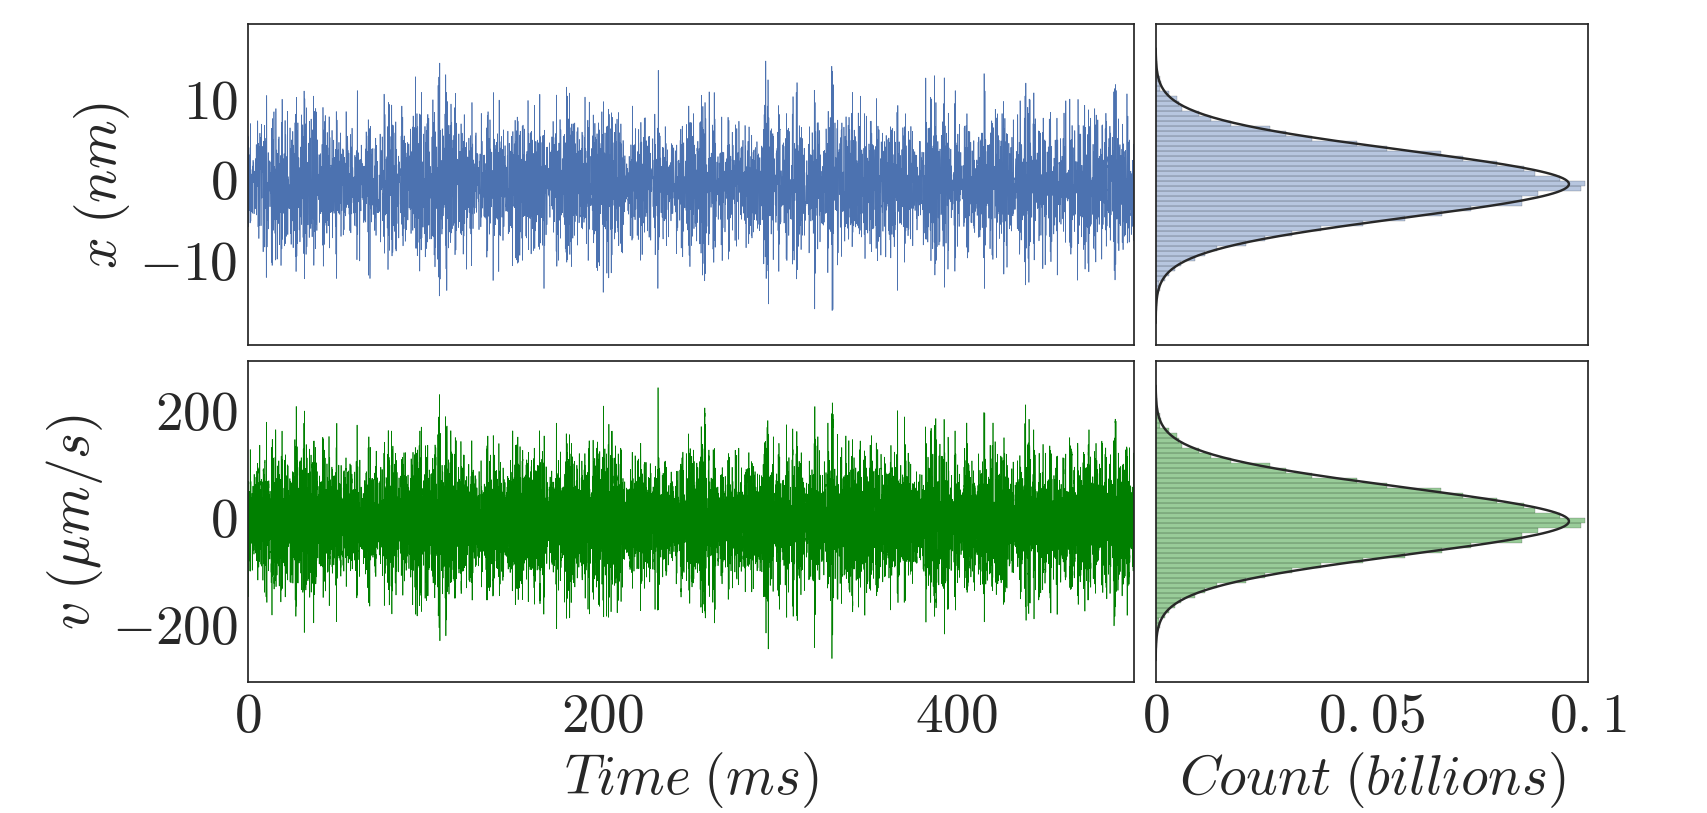
\includegraphics[width=0.48\textwidth]{Fig1}\caption{Sample paths (left) and histograms (right) of the position and velocity
of the Brownian harmonic oscillator obtained from exact path sampling,
Eq. (\ref{eq:path-sampling}). Parameters used are $m=1$ng, $k=225$mg/$s^{2}$,
$\gamma=\gamma_{c}/10$, $\gamma_{c}=\sqrt{4mk}$ and $T=275K$. The
path is sampled at $2^{16}$ Hz. \label{fig:PositionsVelocity}}
\end{figure}
\begin{table*}
\begin{tabular}{|>{\centering}p{2cm}|>{\centering}p{2cm}|>{\centering}p{2cm}|}
\hline 
\multicolumn{3}{|c|}{$m\;\big(ng\big)$}\tabularnewline
\hline 
Simulation & Bayes I & Bayes II\tabularnewline
\hline 
\hline 
$1$ & $0.994\pm0.006$ & $0.993\pm0.008$\tabularnewline
\hline 
$1.5$ & $1.521\pm0.014$ & $1.517\pm0.012$\tabularnewline
\hline 
$2$ & $2.107\pm0.015$ & $2.092\pm0.016$\tabularnewline
\hline 
\end{tabular}%
\begin{tabular}{>{\centering}p{2cm}|>{\centering}p{2cm}|>{\centering}p{2cm}|>{\centering}p{2cm}|>{\centering}p{2cm}|}
\hline 
\multicolumn{3}{c|}{$k\;(mg/s^{2})$} & \multicolumn{2}{c|}{$\gamma\;(\mu g/s^{2})$}\tabularnewline
\hline 
Simulation & Bayes I & Bayes II & Simulation & Bayes I\tabularnewline
\hline 
\hline 
$225$ & $224.81\pm1.72$ & $224.49\pm1.75$ & $3$ & $2.966\pm0.021$\tabularnewline
\hline 
$250$ & $251.97\pm1.93$ & $251.82\pm1.97$ & $1.936$ & $1.974\pm0.016$\tabularnewline
\hline 
$300$ & $316.41\pm2.37$ & $314.88\pm2.46$ & $1.639$ & $1.788\pm0.015$\tabularnewline
\hline 
\end{tabular}

\caption{Bayesian MAP estimates and standard errors of the parameters of the
Brownian harmonic oscillator. There is excellent agreement between
the two Bayesian methods and with the parameter values used to generate
the paths. \label{tab:springconstant}}
\end{table*}

\emph{Parameter estimation: }We now take the time series $\boldsymbol{X}=(x_{1}v_{1},\ldots,x_{N}v_{N})$
of discrete observations of positions and velocities obtained from
the exact path sampling and construct from it the sufficient statistics\begin{subequations}\label{eq:bho-T-matrices}
\begin{alignat}{1}
\boldsymbol{T}_{1} & =\sum_{n=1}^{N-1}\begin{pmatrix}x_{n+1}^{2} & x_{n+1}v_{n+1}\\
v_{n+1}x_{n+1} & v_{n+1}^{2}
\end{pmatrix},\\
\boldsymbol{T}_{2} & =\sum_{n=1}^{N-1}\begin{pmatrix}x_{n+1}x_{n} & x_{n+1}v_{n}\\
v_{n+1}x_{n} & v_{n+1}v_{n}
\end{pmatrix},\\
\boldsymbol{T}_{3} & =\sum_{n=1}^{N-1}\begin{pmatrix}x_{n}^{2} & x_{n}v_{n}\\
v_{n}x_{n} & v_{n}^{2}
\end{pmatrix}.
\end{alignat}
\end{subequations}From these, we compute the MAP estimate for the
regression matrix
\[
\boldsymbol{\lambda}^{\ast}=-\frac{1}{\Delta t}\ln\boldsymbol{\Lambda}^{\ast}=-\frac{1}{\Delta t}\ln(\bm{T}_{2}\boldsymbol{T}_{3}^{-1}),
\]
which yields the MAP estimates for the natural frequency and the relaxation
time scale
\begin{equation}
\left(\frac{k}{m}\right)^{\ast}=\lambda_{21}^{\ast},\quad\left(\frac{\gamma}{m}\right)^{\ast}=\lambda_{22}^{\ast}.
\end{equation}
The MAP estimate of the covariance matrix
\[
\boldsymbol{c}^{\ast}=\dfrac{1}{N}\left(\bm{T}_{1}-\boldsymbol{T}_{2}\boldsymbol{T}_{3}^{-1}\boldsymbol{T}_{2}^{T}\right)\left[\boldsymbol{1}-(\bm{T}_{2}\boldsymbol{T}_{3}^{-1}\boldsymbol{\epsilon})^{T}(\bm{T}_{2}\boldsymbol{T}_{3}^{-1}\boldsymbol{\epsilon})^{T}\right]^{-1}
\]
yields the MAP estimate of the spring constant and the mass, in units
of $k_{B}T$
\begin{equation}
\frac{k_{B}T}{k^{*}}=c_{11}^{\ast},\qquad\frac{k_{B}T}{m^{*}}=c_{22}^{\ast}.
\end{equation}
The friction constant is estimated by eliminating the mass between
two of the previous ratios
\begin{equation}
\gamma^{\ast}=\frac{k_{B}T\lambda_{22}^{\ast}}{c_{22}^{\ast}}.
\end{equation}
The three preceding equations provide the Bayes I map estimates of
the oscillator parameters. 
\begin{figure}
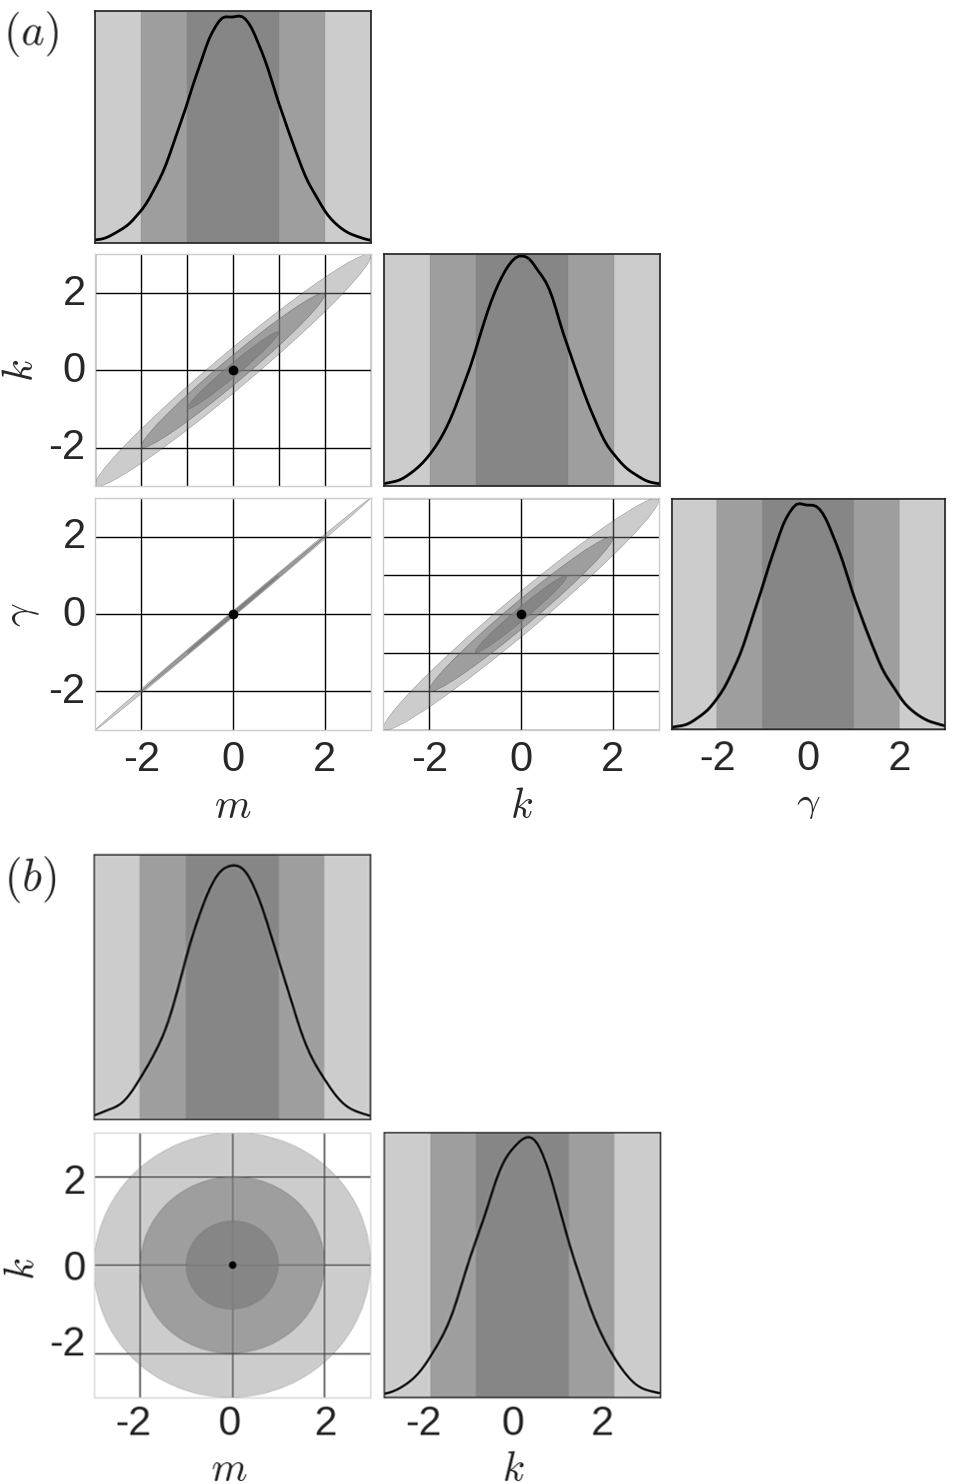
\includegraphics[width=0.45\textwidth]{Fig2}\caption{Corner plots of the joint posterior distribution of the mass $m$,
friction $\gamma$ and stiffness $k$. Panel $(a)$ shows Bayes I,
Eq.(\ref{eq:mapBayesI}) while panel $(b)$ shows Bayes II, Eq.(\ref{eq:map_stationary}).
The variables have been scaled as $\left(x_{i}-\mu_{_{i}}\right)/\sigma_{_{ii}}$,
where $\mu_{i}$ and $\sigma_{ii}^{2}$ are the MAP estimate and variance
of $x_{i}$ respectively. The MAP estimate is marked by a black dot,
and the regions of $70\%$, $90\%$ and $99\%$ posterior probability
have been shaded. \label{fig:inference}\label{fig:stationary}}
 
\end{figure}

Next we use Eq.(\ref{eq:covarianceDiagonal}) for the covariance matrix
in the bivariate analogue of Eq.(\ref{eq:posteriorBayesII}) for the
logarithm of the posterior probability. The MAP estimates and the
error bars for mass $m$ and spring constant $k$ are then\begin{subequations}\label{eq:map_stationary}
\begin{align}
\dfrac{k^{\ast}}{k_{B}T}=\dfrac{N}{\sum_{n=1}^{N}x_{n}^{2}} & ,\qquad\sigma_{k}=\frac{\sqrt{2}}{\sqrt{N}}k^{\ast},\label{eq:map_k}\\
\dfrac{m^{\ast}}{k_{B}T}=\dfrac{N}{\sum_{n=1}^{N}v_{n}^{2}}, & \qquad\,\,\sigma_{m}=\frac{\sqrt{2}}{\sqrt{N}}m^{\ast}.\label{eq:map_v}
\end{align}
\end{subequations}These correspond to Bayes II estimates of the oscillator
parameters. 
\begin{figure}
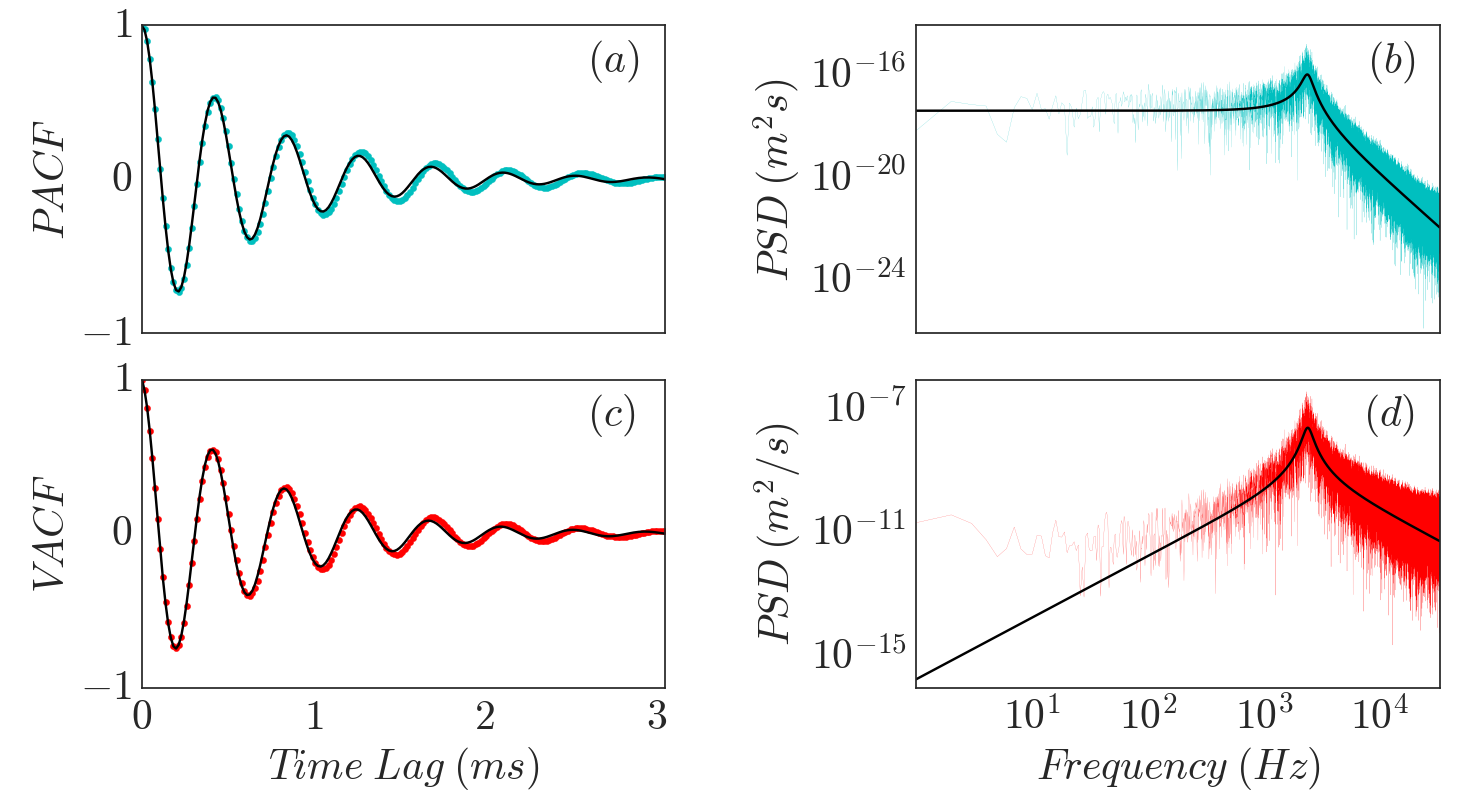
\includegraphics[width=0.46\textwidth]{Fig3}

\caption{Bayesian estimates of the autocorrelation function and spectral density
of position are shown in (a) and (b) respectively as solid lines.
There is excellent agreement with simulations shown in cyan. Corresponding
estimates for the velocity are shown in (c) and (d) with simulations
shown in red. \label{fig:autocorrelation} }
\end{figure}

In Table \ref{tab:springconstant}, we provide the MAP estimates and
corresponding error bars for three different time series data obtained
from the simulation of the underdamped Brownian harmonic oscillator.
This clearly shows that the MAP estimates of both Bayesian methods
and values of the simulation parameters are in excellent agreement.
The error bars have been calculated from the Hessian matrix. The Bayesian
standard error in estimating the parameters is less than $1\%$ for
each case.

In Fig.(\ref{fig:inference}) we show the posterior distribution of
the parameters as corner plots \cite{foreman2016corner}, with panel
(a) corresponding to Bayes I and panel (b) to Bayes II. The distributions
have been shifted to the MAP estimates, which, therefore are always
at the origin marked by the black dot, and scaled by the variances.
The Bayesian credible intervals corresponding to $70\%$, $90\%$
and $99\%$ of the posterior probability are shown in shades of gray. 

\emph{Correlation functions and spectral densities: }The MAP estimates
of the parameters provide a novel way of estimating the correlation
functions and spectral densities. Their expressions can be obtained
from Eq.(\ref{eq:autocorr}) and Eq.(\ref{eq:spectral-density}) using
the explicit forms of the covariance and the regression matrices.
The autocorrelations are 
\begin{align*}
\langle x\left(t\right)x\left(0\right)\rangle= & \dfrac{k_{B}T}{k}\exp\left(\dfrac{-t}{2\tau}\right)\dfrac{(2\omega\tau\cos\omega t+\sin\omega t)}{2\omega\tau},\\
\langle v\left(t\right)v\left(0\right)\rangle= & \dfrac{k_{B}T}{m}\exp\left(\dfrac{-t}{2\tau}\right)\dfrac{(2\omega\tau\cos\omega t-\sin\omega t)}{2\omega\tau}.
\end{align*}
and the spectral densities are
\begin{align*}
C_{xx}(\Omega)= & \dfrac{2\gamma k_{B}T}{m^{2}(\omega_{0}^{2}-\Omega^{2})^{2}+\gamma^{2}\Omega^{2}},\\
C_{vv}(\Omega)= & \dfrac{2\gamma k_{B}T\Omega^{2}}{m^{2}(\omega_{0}^{2}-\Omega^{2})^{2}+\gamma^{2}\Omega^{2}}.
\end{align*}
These expressions are evaluated at the Bayesian MAP estimates for
the parameters. In Fig.(\ref{fig:autocorrelation}) the result is
compared with the autocorrelation function and the discrete Fourier
transform of the time series. There is excellent agreement between
the two autocorrelations. We emphasize that no numerical function
fitting is required to obtain this estimate. The spectral density
is, arguably, even more impressive as it interpolates through the
noisy discrete Fourier transform in a sensible manner. Our estimation
of the spectral density shares a methodological similarity with Burg's
classic maximum entropy method \cite{burg1967maximum}. The principle
differences are (i) that we choose the Ornstein-Uhlenbeck process
as the data generating model, rather than the discrete autoregressive
process assumed by Burg and (ii) that we work directly on the space
of trajectories rather than in the space of correlations. From a Bayesian
perspective, our estimation procedure encodes the prior information
that the data is generated by an Ornstein-Uhlenbeck process and, therefore,
will outperform all methods \cite{berg2004power,tassieri2012microrheology}
that do not incorporate this prior information, such as the one in
\cite{Bera:16}.
\begin{figure}[t]
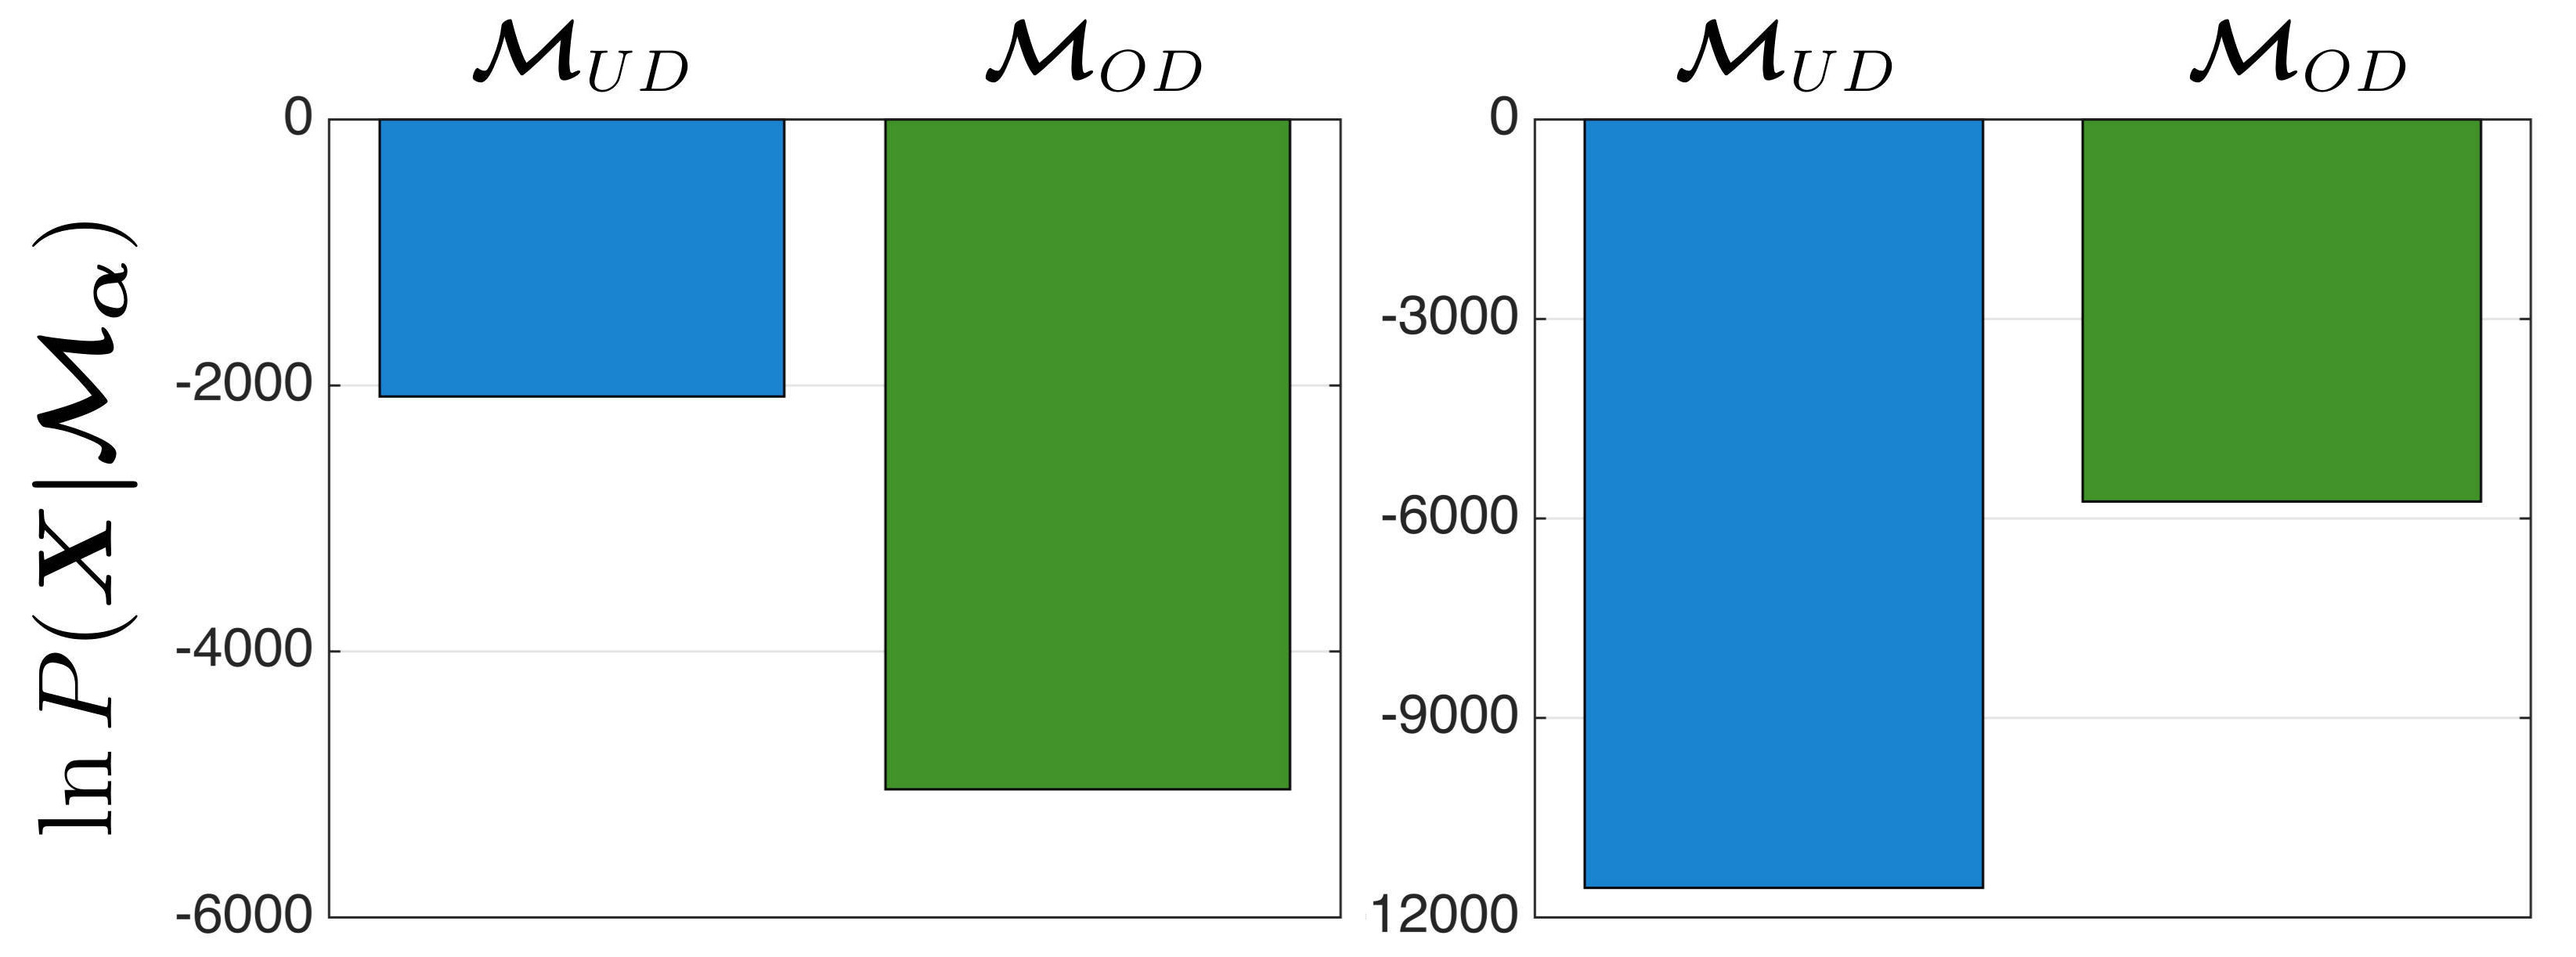
\includegraphics[width=0.46\textwidth]{Fig4.png}

\caption{Bayesian model selection procedure for time series data from underdamped
($\mathcal{M}_{UD}$) and overdamped ($\mathcal{M}_{OD}$) Brownian
harmonic oscillator. The logarithm of Bayesian evidence has been plotted
in the natural log units (nits). The plot for underdamped data $(\gamma=\gamma_{c}/10)$
is shown on the left, while the right panel is for overdamped data
$(\gamma=10\gamma_{c})$.\label{fig:modelSelection} }
\end{figure}

\emph{Model comparison: }To observe the inertial motion of a colloidal
particle in an optical trap, it is necessary to observe the motion
at time intervals much smaller than the momentum relaxation time,
that is, to ensure $\Delta t\ll\tau$. In the opposite limit, of $\Delta t\gg\tau$,
the inertia of the colloid is no longer relevant and only purely diffusive
motion can be observed. These correspond, respectively, to the Kramers
and Smoluchowski limits of the Brownian harmonic oscillator. In experiment,
it is often not a priori clear if the observational time scale places
the system in the Kramers, Smoluchowski or crossover regime. Bayesian
model comparison provides a principled way to answer this question,
as we show below. 

We consider two Ornstein-Uhlenbeck data generating models
\begin{align}
\mathcal{M}_{UD}:\longrightarrow & \quad m\dot{v}+\gamma v+\nabla U=\xi\nonumber \\
\mathcal{M}_{OD}:\longrightarrow & \quad\gamma\dot{x}+\nabla U=\xi
\end{align}
corresponding, respectively, to motion on the Kramers\textbf{\emph{
}}(\textbf{u}nder\textbf{d}amped) and Smoluchoswki (\textbf{o}ver\textbf{d}amped)
time scales. The latter is the formal $m\rightarrow0$ limit of Eq.(\ref{eq:langevin})
and can be obtained systematically by adiabatically eliminating the
velocity as a fast variable \cite{gardiner1984adiabatic}. The overdamped
oscillator is an univariate Ornstein-Uhlenbeck model with two parameters,
$\gamma$ and $k$, and Bayesian parameter estimation for it was presented
in \cite{bera2017fast}. The two-parameter overdamped model is simpler
than the three-parameter underdamped model. The question we try to
answer is which of these models provides the best explanation of the
data for the least number of parameters. 

To do so, we compare the posterior probability of the model, given
the data, by approximating the model evidence in terms of the maximum
likelihood and the Ockham factors, assuming equal prior probabilities
for the models as in section \ref{sec:Bayesian-inference}. The evidence
for both models is straightforwardly computed from the general expression
in the Appendix. For the overdamped model the sufficient statistics
are the scalars
\begin{alignat}{1}
T_{1} & =\sum_{n=1}^{N-1}x_{n+1}^{2},\,\,T_{2}=\sum_{n=1}^{N-1}x_{n+1}x_{n},\,\,T_{3}=\sum_{n=1}^{N-1}x_{n}^{2}.
\end{alignat}
as was first pointed out in \cite{bera2017fast}. 

In Fig.(\ref{fig:modelSelection}), we plot the logarithm of the Bayesian
evidence $\ln P(\boldsymbol{X}|\mathcal{M}_{\alpha})$ in the natural
log units (nits) for overdamped and underdamped Brownian motion. The
panel on the left contains the plot of the logarithm of the evidence
for an underdamped data while the right panel is for an overdamped
data. The comparison of the $\ln P(\boldsymbol{X}|\mathcal{M}_{\alpha})$
for overdamped and underdamped model clearly shows that the evidence
is higher in each case for the true model of the data. 

\section{Summary\label{sec:conclusion}}

In summary, we have presented two Bayesian methods for inferring the
parameters of a multivariate Ornstein-Uhlenbeck process, given discrete
observations of the sample paths. An exact path sampling procedure
has been presented and utilized to validate the Bayesian methods for
the Brownian harmonic oscillator. The problem of Bayesian model comparison
has been addressed and applied to select between Kramers and Smoluchowski
limits of the Brownian harmonic oscillator. Future work will address
the problem of parameter inference and model selection when either
or both of the Markov and Gaussian properties of the process are relaxed.

\widetext

\section*{appendix\label{sec:appendix}}

\subsection*{MAP estimates}

Consider the quadratic form $\bm{\Delta_{n}^{T}\Sigma^{-1}\Delta_{n}}=\left(\bm{x_{n+1}}-\bm{\Lambda}\bm{x_{n}}\right)^{\bm{T}}\bm{\Sigma^{-1}}\left(\bm{x_{n+1}}-\bm{\Lambda}\bm{x_{n}}\right)$
that occurs in the expression of the logarithm of the posterior probability
in Eq.(\ref{eq:posteriorBayesI}). Expanding terms and completing
the summation we have the following identity
\begin{align}
 & -\frac{1}{2}\sum_{n=1}^{N-1}\bm{\Delta_{n}^{T}\Sigma^{-1}\Delta_{n}}=-\dfrac{1}{2}\bm{\Sigma}^{-1}:\Big[\left(\bm{\Lambda}-\bm{T_{2}T_{3}^{-1}}\right)\left(\bm{T_{3}}\right)\left(\bm{\Lambda}-\bm{T_{2}T_{3}^{-1}}\right)^{\bm{T}}+\left(\bm{T_{1}}-\bm{T_{2}T_{3}^{-1}T_{2}^{T}}\right)\Big].\label{eq:lp}
\end{align}
Here, we have used the definitions of sufficient statistics in Eq.
(\ref{eq:sufficientStatistics}). With this identification, the expression
of the logarithm of the posterior probability in terms of the sufficient
statistics is
\begin{align}
\ln P\left(\bm{\theta}\vert\bm{X}\right)= & -\dfrac{1}{2}\bm{\Sigma}^{-1}:\Big[\left(\bm{\Lambda}-\bm{T_{2}T_{3}^{-1}}\right)\left(\bm{T_{3}}\right)\left(\bm{\Lambda}-\bm{T_{2}T_{3}^{-1}}\right)^{\bm{T}}+\left(\bm{T_{1}}-\bm{T_{2}T_{3}^{-1}T_{2}^{T}}\right)\Big]+\frac{N}{2}\ln\dfrac{|\bm{\Sigma^{-1}}|}{(2\pi)^{M}}.
\end{align}
Inspecting the above expression, we recognize that the posterior is
normal in $\boldsymbol{\Lambda}$ which directly yields its MAP estimate
$\boldsymbol{\Lambda^{\ast}}=\bm{T_{2}T_{3}^{-1}}$. Taking the derivative
of above equation with respect to $\boldsymbol{\Sigma}^{-1}$ and
using the matrix identity $\partial\ln\left(\det\bm{A}\right)/\partial\bm{A}=\left(\bm{A}^{T}\right)^{-1}$,
we obtain
\begin{align}
 & \dfrac{\partial\ln P\left(\bm{\theta}\vert\bm{X}\right)}{\partial\bm{\Sigma^{-1}}}=-\dfrac{1}{2}\Big[\left(\bm{\Lambda}-\bm{T_{2}T_{3}^{-1}}\right)\left(\bm{T_{3}}\right)\left(\bm{\Lambda}-\bm{T_{2}T_{3}^{-1}}\right)^{\bm{T}}+\left(\bm{T_{1}}-\bm{T_{2}T_{3}^{-1}T_{2}^{T}}\right)\Big]+\dfrac{N}{2}\bm{\Sigma}.
\end{align}
At the maximum, we obtain the MAP estimate as $\bm{\Sigma^{\ast}}=\dfrac{1}{N}\left(\bm{T}_{1}-\boldsymbol{T}_{2}\boldsymbol{T}_{3}^{-1}\boldsymbol{T}_{2}^{T}\right).$
The estimates of the parameters of the underdamped oscillator follow
from $\bm{\Lambda^{\ast}}$ and $\bm{\Sigma^{\ast}}$ after algebraic
manipulations. 

\subsection*{Standard errors and evidence}

The second partial derivatives of the logarithm of the posterior distribution
with respect to $\boldsymbol{\Sigma}^{-1}$ and $\boldsymbol{\Lambda}$,
at the maximum, are\begin{subequations}
\begin{align}
\dfrac{\partial^{2}\ln P\left(\bm{\theta}\vert\bm{X}\right)}{\partial(\bm{\Sigma^{-1}})^{2}}= & -\dfrac{N}{2}\left(\bm{\Sigma}^{*}\right)^{2},\\
\dfrac{\partial^{2}\ln P\left(\bm{\theta}\vert\bm{X}\right)}{\partial\bm{\Lambda}^{2}}= & -\bm{\Sigma}^{*-1}(\bm{T_{3}}+N\boldsymbol{c}*)-\frac{N}{2}\bm{\Sigma}^{*-2}((\bm{\Lambda}^{*}\boldsymbol{c}^{*}+\boldsymbol{c}^{*}\bm{\Lambda}^{*T}))^{2}.
\end{align}
\end{subequations}The mixed partial derivative at the maximum is
\begin{align}
\dfrac{\partial^{2}\ln P\left(\bm{\theta}\vert\bm{X}\right)}{\partial\bm{\Lambda}\partial\bm{\Sigma^{-1}}} & \eqsim-\frac{N}{2}(\bm{\Lambda}^{*}\boldsymbol{c}^{*}+\boldsymbol{c}^{*}\bm{\Lambda}^{*T}).
\end{align}
The Hessian matrix, $\boldsymbol{A}=-\nabla\nabla\ln P\left(\bm{\theta}\vert\bm{X}\right)$,
at the maximum is then
\begin{align}
 & \boldsymbol{A}=\left(\begin{array}{ccc}
\tfrac{N}{2}(\bm{\Sigma}^{*})^{2} & \qquad & \frac{N}{2}(\bm{\Lambda}^{*}\boldsymbol{c}^{*}+\boldsymbol{c}^{*}\bm{\Lambda}^{*T})\\
 & \qquad\\
\frac{N}{2}(\bm{\Lambda}^{*}\boldsymbol{c}^{*}+\boldsymbol{c}^{*}\bm{\Lambda}^{*T})\, & \qquad & \bm{\Sigma}^{*-1}(\bm{T_{3}}-N\boldsymbol{c}^{*})-\frac{N}{2}\bm{\Sigma}^{*-2}(\bm{\Lambda}^{*}\boldsymbol{c}^{*}+\boldsymbol{c}^{*}\bm{\Lambda}^{*T})^{2}
\end{array}\right).
\end{align}
The above expression of the Hessian matrix have been used to obtain
the standard errors of the MAP estimates and the evidence of a given
model.

The expression of the Bayesian evidence of a model $\mathcal{M}_{\alpha}$
with several parameters is given in terms of the likelihood and the
Hessian matrix as \cite{mackay2003information}
\begin{equation}
P(\boldsymbol{X}|\mathcal{M}_{\alpha})\simeq P(\boldsymbol{X}|\boldsymbol{\theta}^{\ast},\mathcal{M}_{\alpha})\,P(\boldsymbol{\theta}^{\ast}|\mathcal{M}_{\alpha})[\det(\bm{A}/2\pi)]^{-1/2}.\label{eq:evidence-multivariate-1}
\end{equation}
This expression has been used to obtain the logarithm of the evidence
for a $M$-dimensional multivariate Ornstein-Uhlenbeck model $\mathcal{M}_{\alpha}$.
Using explicit forms of the likelihood and the Hessian matrix, at
the maximum, the expression of the logarithm of the evidence for a
model $\mathcal{M}_{\alpha}$ is given as
\begin{align}
\ln P\left(\bm{X}|\mathcal{M}_{\alpha}\right) & \simeq-\frac{N}{2}\left(\bm{\Sigma}^{*^{-1}}:\bm{\Sigma}^{*}+\ln((2\pi)^{M}\,|\bm{\Sigma}^{*}|)\right)-\frac{1}{2}\ln\Big(\det(\boldsymbol{A}_{22})\det(\boldsymbol{A}_{11}-\boldsymbol{A}_{12}\boldsymbol{A}_{22}^{-1}\boldsymbol{A}_{21})\Big)+\tfrac{M}{2}\ln2\pi.
\end{align}
Here $\boldsymbol{A}_{ij}$ are the elements of the Hessian matrix.
%
%
\begin{thebibliography}{10}

\bibitem{gardiner1985handbook}
C.~W. Gardiner.
\newblock {\em Handbook of stochastic methods}.
\newblock Springer Berlin, 1985.

\bibitem{van1992stochastic}
N.~G. van Kampen.
\newblock {\em Stochastic processes in physics and chemistry}.
\newblock Elsevier, 1992.

\bibitem{jeffreys1998theory}
H.~Jeffreys.
\newblock {\em The theory of probability}.
\newblock Oxford University Press, Oxford, 1939.

\bibitem{jaynes2003probability}
E.~T. Jaynes.
\newblock {\em Probability theory: The logic of science}.
\newblock Cambridge University Press, 2003.

\bibitem{sivia2006data}
D.~Sivia and J.~Skilling.
\newblock {\em Data analysis: a {B}ayesian tutorial}.
\newblock Oxford University Press, Oxford, 2006.

\bibitem{bera2017fast}
S.~Bera, S.~Paul, R.~Singh, D.~Ghosh, A.~Kundu, A.~Banerjee, and R.~Adhikari.
\newblock Fast {B}ayesian inference of optical trap stiffness and particle
  diffusion.
\newblock {\em Sci. Rep.}, 7:41638, 2017.

\bibitem{kashyap1977bayesian}
R.~Kashyap.
\newblock A bayesian comparison of different classes of dynamic models using
  empirical data.
\newblock {\em IEEE Trans. Automat. Cont.}, 22(5):715--727, 1977.

\bibitem{mackay1992bayesian}
D.~J.~C. MacKay.
\newblock Bayesian interpolation.
\newblock {\em Neur. Computn.}, 4:415--447, 1992.

\bibitem{zellner1984}
A.~Zellner.
\newblock {\em Basic Issues in Econometrics}.
\newblock University of Chicago Press, Chicago, 1984.

\bibitem{gregory2005bayesian}
P.~Gregory.
\newblock {\em Bayesian Logical Data Analysis for the Physical Sciences}.
\newblock Cambridge University Press, 2005.

\bibitem{uhlenbeck1930theory}
G.~E. Uhlenbeck and L.~S. Ornstein.
\newblock On the theory of the brownian motion.
\newblock {\em Phys. Rev.}, 36(5):823, 1930.

\bibitem{chandrasekhar1943stochastic}
S.~Chandrasekhar.
\newblock Stochastic problems in physics and astronomy.
\newblock {\em Rev. Mod. Phys.}, 15:1--89, 1943.

\bibitem{einstein1905theory}
A.~Einstein.
\newblock The theory of the {B}rownian movement.
\newblock {\em Ann. Phys. (Berlin)}, 322:549, 1905.

\bibitem{kubo1966fluctuation}
R.~Kubo.
\newblock The fluctuation-dissipation theorem.
\newblock {\em Rep. Prog. Phys.}, 29(1):255, 1966.

\bibitem{foreman2016corner}
D.~Foreman-Mackey.
\newblock corner.py: Scatterplot matrices in {P}ython.
\newblock {\em The Journal of Open Source Software}, 1(2):1--2, 2016.

\bibitem{burg1967maximum}
J.~P. Burg.
\newblock Maximum entropy spectral analysis.
\newblock In {\em 37th Meeting, Soc. of Explor. Geophys., Oklahoma City}, 1967.

\bibitem{berg2004power}
K.~Berg-S{\o}rensen and H.~Flyvbjerg.
\newblock Power spectrum analysis for optical tweezers.
\newblock {\em Rev. Sci. Inst.}, 75(3):594--612, 2004.

\bibitem{tassieri2012microrheology}
M.~Tassieri, R.~Evans, R.~L. Warren, N.~J. Bailey, and J.~M. Cooper.
\newblock Microrheology with optical tweezers: data analysis.
\newblock {\em New J. Phys.}, 14(11):115032, 2012.

\bibitem{Bera:16}
S.~Bera, A.~Kumar, S.~Sil, T.~K. Saha, T.~Saha, and A.~Banerjee.
\newblock Simultaneous measurement of mass and rotation of trapped absorbing
  particles in air.
\newblock {\em Opt. Lett.}, 41(18):4356--4359, 2016.

\bibitem{gardiner1984adiabatic}
C.~W. Gardiner.
\newblock Adiabatic elimination in stochastic systems. i. formulation of
  methods and application to few-variable systems.
\newblock {\em Phys. Rev. A}, 29(5):2814--2822, 1984.

\bibitem{mackay2003information}
D.~J.~C. MacKay.
\newblock {\em Information theory, inference and learning algorithms}.
\newblock Cambridge University Press, 2003.

\end{thebibliography}
\end{document}
